\chapter{Derivate parțiale}
\index{derivate parțiale}

În general, putem lucra cu funcții de mai multe variabile, sub forma
$ f : \RR^n \to \RR $, funcții care acceptă $ n $ variabile ca \qq{date de intrare}
și rezultatul este o variabilă reală, deci $ f(x_1, \dots, x_n) = y \in \RR $,
pentru orice $ n $-tuplu $ (x_1, \dots, x_n) \in \RR^n $.

Cazurile pe care le vom întîlni cel mai des la acest seminar vor fi, însă,
$ n = 2 $ și $ n = 3 $, cazuri în care variabilele de intrare se vor nota,
respectiv $ (x, y) $ sau $ (x, y, z) $.

Fie, deci, $ f : \RR^3 \to \RR $ o funcție de 3 variabile reale, cu valori
reale, $ f = f(x, y, z) $.

Putem defini \emph{derivata parțială} a funcției $ f $ după variabila $ x $,
de exemplu, ca fiind derivata obținută prin tratarea lui $ y $ și $ z $ ca
parametri (\qq{constante}). Notația este $ \dfrac{\partial f}{\partial x} $
sau $ f_x $ sau $ \partial_x f $.

Similar se pot defini și celelalte derivate parțiale. Un exemplu simplu:
\[
  f : \RR^3 \to \RR, \quad f(x, y, z) = 3x^2 y + 5xe^y + \sin(yz).
\]

Avem:
\begin{align*}
  f_x &= 6xy + 5e^y \\
  f_y &= 3x^2 + 5xe^y + z \cos(yz) \\
  f_z &= y\cos(yz).
\end{align*}

Calculele pot continua și putem defini \emph{derivatele parțiale de ordin %
  superior}:
\[
  f_{xx} = \dfrac{\partial^2 f}{\partial x^2} = %
  \dfrac{\partial}{\partial x} \left( \dfrac{\partial f}{\partial x} \right)
\]
și similar pentru derivate mixte de forma $ f_{xy}, f_{yx} $ sau derivate de ordin
și mai mare.

În cazul funcțiilor pe care le vom folosi, are loc:
\begin{theorem}[Teorema de simetrie a lui Schwarz]\label{thm:schwarz}\index{teorema!Schwarz}
  În anumite ipoteze\footnotemark, derivatele mixte au proprietatea de simetrie,
  adică $ f_{x_i x_j} = f_{x_j x_i} $ sau, scris pe larg:
  \[
    \dfrac{\partial^2 f}{\partial x_i \partial x_j} = \dfrac{\partial^2 f}{\partial x_j \partial x_i},%
    \forall x_i, x_j.
  \]
\end{theorem}
\footnotetext{O prezentare a teoremei se poate găsi \href{https://en.wikipedia.org/wiki/Symmetry\_of\_second\_derivatives\#Schwarz.27s\_theorem}{aici},
  iar în exercițiile de la seminar, ipotezele vor fi verificate automat.}

În exercițiile pe care le vom aborda, vor fi de folos derivatele de ordinul întîi și
cele de ordinul al doilea. În plus, pentru o funcție de 3 variabile reale,
$ f : \RR^3 \to \RR, f = f(x, y, z) $, se definește \emph{laplacianul} (sau
\emph{operatorul Laplace}) prin:
\index{derivate parțiale!laplacian}
\[
  \Delta f = f_{xx} + f_{yy} + f_{zz}.
\]

Similar, desigur, putem defini laplacianul și pentru funcții de 2 variabile reale prin:
\[
  \Delta f = f_{xx} + f_{yy}.
\]

O funcție se numește \emph{armonică} dacă $ \Delta f = 0 $.
\index{derivate parțiale!funcție armonică}

\vspace{1cm}

Dată o funcție de 3 variabile, se poate defini \emph{diferențiala totală},
care conține laolaltă informațiile furnizate de derivatele parțiale. Pentru o
funcție $ f : \RR^3 \to \RR $, diferențiala totală se notează $ df $ și se calculează
cu formula:
\[
  df = f_x dx + f_y dy + f_z dz,
\]
unde $ dx, dy, dz $ sînt diferențialele elementare (nu se calculează! ele
constituie vectori-bază într-un anumit spațiu vectorial).

O expresie ca mai sus, de forma $ df $, se numește \emph{1-formă diferențială},
pe care o vom reîntîlni în studiul integralelor curbilinii.

Avem mai departe și diferențiala totală de ordinul al doilea, definită
pentru aceeași funcție de mai sus prin:
\[
  d^2 f = f_{xx} dx^2 + 2f_{xy} dxdy + f_{yy} dy^2,
\]
expresie care se mai numește \emph{2-formă diferențială} și pe care o
vom reîntîlni în studiul integralelor de suprafață.

\vspace{1cm}

De asemenea, o altă noțiune utilă este aceea a \emph{polinoamelor Taylor}
pentru funcții de mai multe variabile. Fie $ f = f(x, y) $ o funcție
de 2 variabile și fie $ A(x_A, y_A) \in \RR^2 $ un punct arbitrar. În exerciții,
vom întîlni doar polinoamele Taylor de grad 1 și 2, care se definesc astfel,
în jurul punctului $ A $:
\begin{align*}
  T_1(X, Y) &= f(A) + \dfrac{1}{1!}\left[f_x(A)(X - x_A) + f_y(A)(Y - y_A)\right] \\
  T_2(X, Y) &= T_1(X, Y) + \dfrac{1}{2!} \left[ f_{xx}(A)(X - x_A)^2 + f_{yy}(A)(Y - y_A)^2 +%
              2f_{xy}(A)(X - x_A)(Y - y_A) \right].
\end{align*}

Ca în cazul seriilor Taylor pentru funcțiile de o singură variabilă,
eroarea aproximației folosind aceste polinoame este comparabilă cu primul termen neglijat.


%%%%%%%%%%%%%%%%%%%%%%%%%%%%%%%%%%%%%%%%%%%%%%%%%%%%%%%%%%%%%%%%%%%%%% 
\section{Extreme libere}
\index{extreme!libere}

Fie o funcție de 2 variabile $ f : \RR^2 \to \RR, f = f(x, y) $. Ne propunem
să studiem valorile sale extreme, adică să îi găsim minimul și maximul,
considerînd că funcția este definită, derivabilă și continuă pe tot domeniul
de definiție.

Pașii pe care îi urmăm sînt:
\begin{enumerate}[(1)]
\item Rezolvăm sistemul de ecuații dat de anularea derivatelor parțiale
  de ordinul întîi, din care aflăm \emph{punctele critice}, care \emph{este posibil}
  să fie de extrem. Așadar, rezolvăm sistemul:
  \[
    \begin{cases}
      f_x &= 0 \\
      f_y &= 0
    \end{cases} \Longrightarrow A_1(x_1, y_1), A_2(x_2, y_2)\dots
  \]
\item Pentru fiecare dintre punctele critice $ A_i $ se alcătuiește
  \emph{matricea hessiană} a funcției, alcătuită din derivatele de ordinul al
  doilea și se evaluează matricea în punctele critice:
  \[
    H_f(A_i) = \begin{pmatrix}
      f_{xx}(A_i) & f_{xy}(A_i) \\
      f_{yx}(A_i) & f_{yy}(A_i)
    \end{pmatrix}
  \]
  \index{derivate parțiale!matricea hessiană}
\item Fie $ A_i $ un punct critic fixat. Calculăm valorile proprii $ \lambda_{1,2} $ ale
  matricei hessiene $ H_f(A_i) $ și decidem astfel:
  \begin{itemize}
  \item Dacă $ \lambda_1, \lambda_2 > 0 $, atunci punctul $ A_i $ este de \emph{minim local};
  \item Dacă $ \lambda_1, \lambda_2 < 0 $, punctul $ A_i $ este \emph{maxim local};
  \item Dacă $ \lambda_1 \cdot \lambda_2 < 0 $, punctul $ A_i $ \emph{nu este de extrem};
  \item Dacă $ \lambda_1 \cdot \lambda_2 = 0 $, nu putem decide.
  \end{itemize}
\item Se repetă procedura pentru fiecare dintre punctele critice.
\end{enumerate}

\section{Metoda celor mai mici pătrate}

Această metodă este strîns legată de conceptul de \emph{interpolare}, care
ne ajută să găsim cea mai potrivită curbă, pornind de la un set de puncte
(reprezentînd, eventual, date experimentale).

Cazul particular pe care îl vom discuta este acela al curbelor liniare,
deci atunci cînd se caută cea mai potrivită \emph{dreaptă} pentru un set
de puncte. Această dreaptă se mai numește \emph{dreaptă de regresie}
și spunem că ea \emph{mediază} între un set de puncte date, în sensul
că optimizează erorile.
\index{dreaptă!de regresie}

Pe scurt, dacă se dă un set de date experimentale, distribuite într-un
anume fel în plan și avem de găsit cea mai potrivită dreaptă care să
medieze între aceste puncte, sîntem în situația din figura \ref{fig:mcmmp}.

\begin{figure}[!htbp]
  \centering
  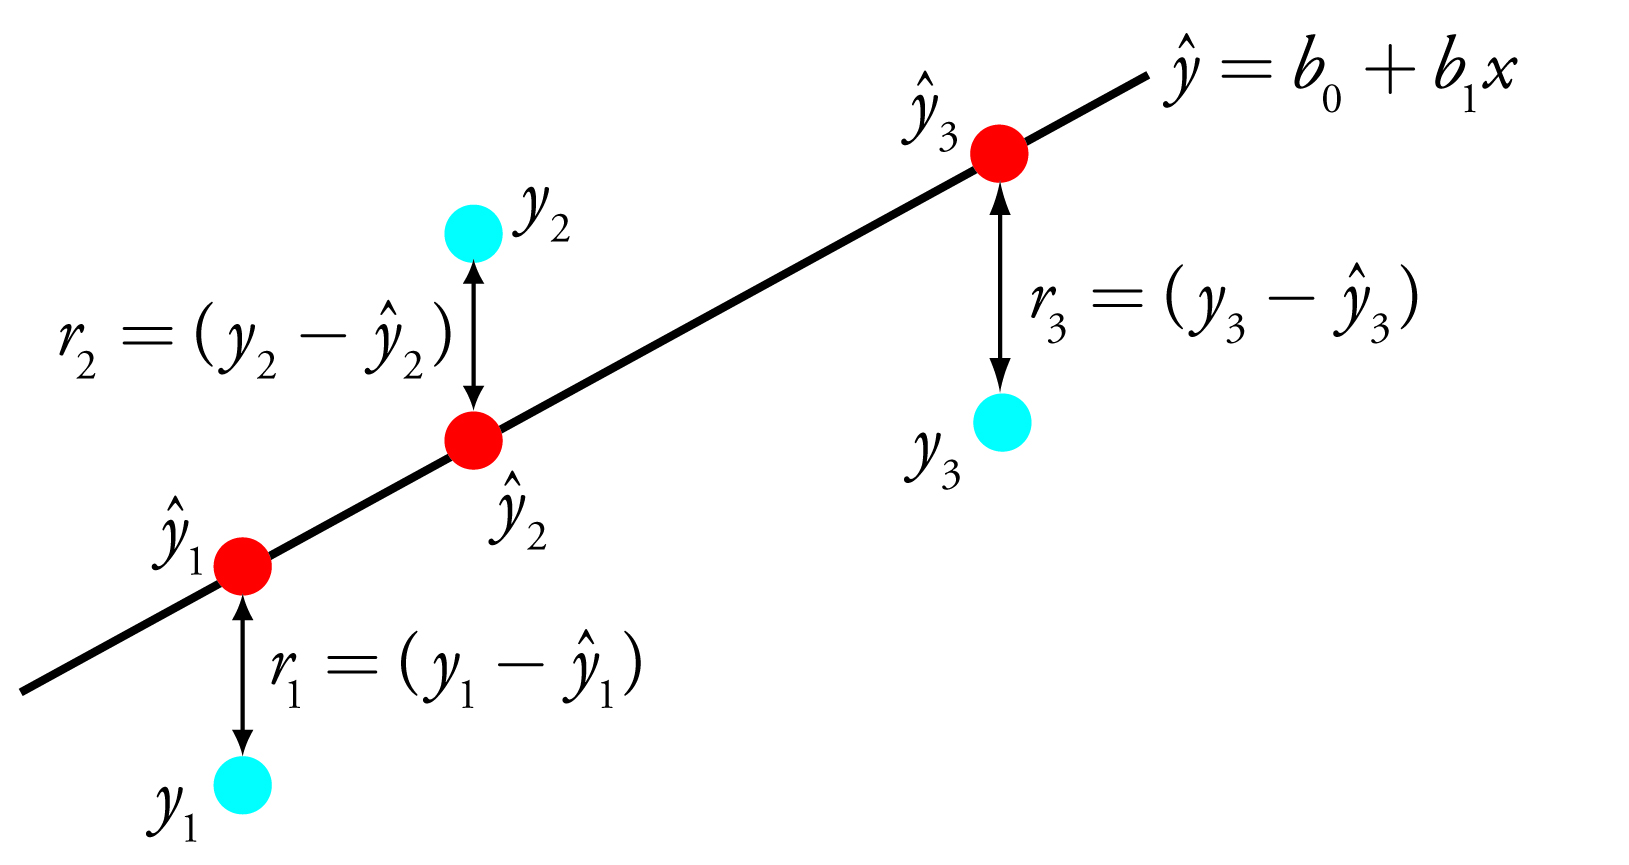
\includegraphics[scale=0.6]{fig/leastsquare.jpg}
  \caption{\emph{Dreapta $ \hat{y} = b_0 + b_1 x $ care mediază \\ %
      între punctele $ y_i $, cu calculul erorilor $ r_i $}}
  \label{fig:mcmmp}
\end{figure}

Această dreaptă se va găsi astfel încît \emph{suma pătratelor erorilor}
să fie minimă. Motivul simplu este că erorile pot fi și pozitive, și
negative, iar mai mult, erorile mari vrem să fie \qq{amplificate} de
metodă, erorile mai mici fiind de o importanță inferioară. De aceea,
metoda se numește \emph{metoda celor mai mici pătrate}.

Fie, deci, dreapta $ y = ax + b $, dreapta de regresie liniară pe care
o căutăm, care să medieze între punctele $ P_i(x_i, y_i) $.

Echivalent, putem scrie relația și funcțional, în sensul că dreapta
căutată se asociază unei funcții $ f(x) = ax + b $. Atunci,
dacă punctul $ P_i $ se găsește pe această dreaptă, are loc relația
$ f(x_i) = y_i $. Rezultă că eroarea poate fi calculată prin diferența
$ |y_i - f(x_i)| $ și vom fi interesați de suma pătratelor acestor erori.
Aceasta va fi funcția pe care încercăm să o minimizăm, iar argumentele sale
sînt coeficienții $ a, b $ care definesc dreapta căutată

Așadar, definim:
\[
  F(a, b) = \sum_i (f(x_i) - y_i)^2 = \sum_i (ax_i + b - y_i)^2.
\]

Metoda dorește, deci, să minimizeze eroarea, deci problema revine la a găsi
$ M(a, b) $ \emph{punctul de minim} al funcției $ F(a, b) $ de mai sus.
Coordonatele punctului vor defini dreapta de regresie căutată.

%%%%%%%%%%%%%%%%%%%%%%%%%%%%%%%%%%%%%%%%%%%%%%%%%%%%%%%%%%%%%%%%%%%%%% 

\section{Funcții implicite}


Funcțiile implicite sînt definite de ecuații care, în general, nu se pot
rezolva sau se rezolvă foarte dificil. De exemplu, dacă avem o ecuație
de forma:
\[
  xy + 2x\sin y = 0
\]
și vrem să exprimăm de aici funcția $ y = y(x) $, constatăm că acest
lucru nu este posibil, deoarece ecuația nu poate fi rezolvată pentru $ y $.
Astfel, vom spune în acest caz că $ y $ a fost definită \emph{implicit}
de ecuația de mai sus.
\index{funcții!implicite}

Trecem direct la exemplificarea noțiunilor teoretice pe exerciții rezolvate.

\vspace{0.5cm}

1. Funcția $ z = z(x, y) $ este definită implicit de ecuația:
\[
  (y + z) \sin z - y (x + z) = 0.
\]
Calculați expresia:
\[
  E = z \sin z \frac{\partial z}{\partial x} - y^2 \frac{\partial z}{\partial y}.
\]

\emph{Soluție:} Notăm expresia implicită dată cu $ F(x, y, z) $. Pentru a putea
exprima $ z = z(x, y) $, deci ca funcție, este necesar ca expresia $ F $ să depindă
\emph{funcțional} de $ z $, adică să nu aibă pe $ z $ doar ca parametru ori drept
constantă. Așadar, avem o \emph{condiție de existență} a funcției implicite
$ z = z(x, y) $, anume $ \dfrac{\partial F}{\partial z} \neq 0 $.

Presupunem acum că ne aflăm în ipoteza de mai sus, i.e.\ condiția de existență
este satisfăcută. Atunci, pentru a exprima $ \dfrac{\partial z}{\partial x} $
și $ \dfrac{\partial z}{\partial y} $, vom deriva expresia $ F $, deoarece
doar acolo apare funcția $ z $. Obținem:
\[
  \frac{\partial F}{\partial x} = \frac{\partial z}{\partial x} \sin z + %
  (y + z) \cos z \dfrac{\partial z}{\partial x} - %
  y\Big(1 + \dfrac{\partial z}{\partial x} \Big) = 0
\]
Rezultă:
\[
  \frac{\partial z}{\partial x} = \frac{z}{\sin z + (y + z) \cos z - y}.
\]

Similar:
\[
  \frac{\partial F}{\partial y} = \Big(1 + \frac{\partial z}{\partial y} \Big) \sin z + %
  (y + z) \cos z \frac{\partial z}{\partial y} - (x + z) - y \frac{\partial z}{\partial y} = 0.
\]
Rezultă:
\[
  \frac{\partial z}{\partial y} = \dfrac{x + z - \sin z}{\sin z + (y + z)\cos z - y}.
\]
Înlocuind în expresia cerută, obținem $ E = 0 $.

\vspace{0.5cm}

Un alt tip de exercițiu de care sîntem interesați este acela al extremelor pentru
funcții definite implicit.

2. Să se determine extremele funcției $ y = y(x) $, definită implicit de ecuația:
\[
  x^3 + y^3 - 2xy = 0.
\]

\emph{Soluție:} Fie $ F(x, y) = x^3 + y^3 - 2xy $, astfel încît condiția dată
este $ F(x, y) = 0 $.

Pentru a extrage funcția $ y = y(x) $, este necesar să punem condiția
de existență:
\[
  \dfrac{\partial F}{\partial y} \neq 0 \Rightarrow 3y^2 - 2x \neq 0.
\]

Acum, știind că avem funcția $ y = y(x) $, extremele acesteia se determină
folosind derivata $ y'(x) $, pe care nu o putem obține altfel decît prin
intermediul funcției $ F $. Avem, așadar:
\[
  \frac{\partial F}{\partial x} = 3x^2 - 3y^2 y' - 2y - 2x y' = 0.
\]
Obținem de aici:
\[
  y'(x) = \frac{2y - 3x^2}{3y^2 - 2x}.
\]
Pentru extreme, avem condițiile:
\[
  \begin{cases}
    y'(x) &= 0 \\
    F(x, y) &= 0 \\
    \dfrac{\partial F}{\partial y} &\neq 0
  \end{cases}
\]

Rezultă $ y = \dfrac{3x^2}{2} $ și înlocuim, obținînd perechea de soluții:
\[
  (x, y) = \Big( \dfrac{2\sqrt[3]{3}}{3}, \dfrac{2\sqrt[3]{4}}{3} \Big).
\]

Pentru a decide natura punctului de mai sus, este necesar să calculăm
$ y^{\prime\prime} $, care se obține derivînd din nou expresia pentru $ y'(x) $.
Avem:
\[
  y^{\prime\prime}(x) = \frac{(2y' - 6x)(3y^2 - 2x) - (6yy' - 2)(2y - 3x^2)}{(3y^2 - 2x)^2}.
\]
Evaluînd pentru $ x = \dfrac{2 \sqrt[3]{2}}{3} $, unde $ y' = 0 $, găsim:
\[
  y^{\prime\prime}\Big( \dfrac{2 \sqrt[3]{2}}{4} \Big) = -3 < 0,
\]
deci punctul este de maxim local.


%%%%%%%%%%%%%%%%%%%%%%%%%%%%%%%%%%%%%%%%%%%%%%%%%%%%%%%%%%%%%%%%%%%%%% 
\section{Exerciții}

1. Verificați dacă următoarele funcții de 2 variabile sînt armonice (presupunem
că domeniile de definiție au fost date corect):
\begin{enumerate}[(a)]
\item $ f(x, y) = \ln(x^2 + y^2) $;
\item $ f(x, y) = \sqrt{x^2 + y^2} $;
\item $ f(x, y) = \arctan \dfrac{x}{y} + \arctan\dfrac{y}{x} $;
\item $ f(x, y) = \dfrac{x + y}{x - y} $.
\end{enumerate}

\vspace{0.3cm}

2. Găsiți punctele de extrem pentru funcțiile de 2 sau 3 variabile, definite
corespunzător pe $ \RR^2 $ sau $ \RR^3 $:
\begin{enumerate}[(a)]
\item $ f(x, y) = 3x^2y - 2x + 5y - xy^2 $;
\item $ f(x, y) = x^3 + y^3 - 6xy $;
\item $ f(x, y) = 3xy^2 - x^3 - 15x - 36y + 9 $;
\item $ f(x, y) = 4xy - x^4 - y^4 $;
\end{enumerate}

\vspace{0.3cm}

3. Arătați că funcțiile următoare verifică ecuațiile indicate:
\begin{enumerate}[(a)]
\item $ f(x, y) = \varphi \Big( \dfrac{y}{x} \Big) $,
  \[
    x \frac{\partial f}{\partial x} + y \frac{\partial f}{\partial y} = 0.
  \]
\item $ f(x, y, z) = \varphi(xy, x^2 + y^2 + z^2) $,
  \[
    xz \frac{\partial f}{\partial x} - yz \frac{\partial f}{\partial y} + %
    (y^2 - x^2) \frac{\partial f}{\partial z} = 0.
  \]
\item $ f(x, y) = y \varphi(x^2 - y^2) $,
  \[
    \frac{1}{x} \frac{\partial f}{\partial x} + \frac{1}{y} \frac{\partial f}{\partial y} = %
    \frac{1}{y^2} f(x, y);
  \]
\item $ f(x, y, z) = \dfrac{xy}{z} \ln x + x\varphi \Big( \dfrac{x}{y}, \dfrac{z}{x} \Big) $,
  pentru $ x > 0 $ și $ z \neq 0 $, ecuația fiind:
  \[
    x \frac{\partial f}{\partial x} + y \frac{\partial f}{\partial y} + z \frac{\partial f}{\partial z} - %
    \frac{xy}{z} - f(x, y, z) = 0.
  \]
\end{enumerate}

\vspace{0.3cm}

4. Găsiți dreptele de regresie care mediază între punctele:
\begin{enumerate}[(a)]
\item $ (1, 3), (2, 4), (-1, 0) $;
\item $ (2, 3), (-1, -1), (0, 2) $;
\item $ (1, 0), (2, 1), (3, 2), (-1, 2) $;
\item $ (1, 1), (2, 1), (-1, 0), (-2, 1) $;
\item $ (1, 0), (2, 1), (-1, 1), (-2, -2) $.
\end{enumerate}

\vspace{0.3cm}

5. Fie funcția $ z = z(x, y) $, definită implicit prin:
\[
  g(y^2 - x^2, z - xy) = 0,
\]

unde $ g \in \kal{C}^1(\RR^2) $. Calculați expresia:
\[
  E = y \dfrac{\partial z}{\partial x} + x \dfrac{\partial z}{\partial y}.
\]

\vspace{0.3cm}

6. Să se determine extremele funcției $ y = y(x) $, definită implicit
de ecuațiile:
\begin{enumerate}[(a)]
\item $ x^3 + y^3 - 3x^2y - 3 = 0 $;
\item $ 2x^2y + y^2 - 4x - 3 = 0 $;
\item $ (x^2 + y^2)^2 = x^2 - y^2 $;
\item $ x^2 - 2xy + 5y^2 - 2x + 4y = - 1 $;
\item $ x^2 + y^2 - e^{2 \arctan \frac{x}{y}} = 0 $.
\end{enumerate}

\vspace{0.3cm}

7. Fie funcția $ z = z(x, y) $, definită implicit de ecuația:
\[
  F(x, y, z) = x^2 + 2y^2 + z^2 - 4z = 12.
\]
Să se calculeze derivatele parțiale de ordinul întîi și al doilea
pentru funcția $ z $.


%%% Local Variables:
%%% mode: latex
%%% TeX-master: "../am1-20-21"
%%% End:
